\begin{pastexam}[label={px:nccu-107-dsa-08}]{政大資科所 107 學年度 第 8 題}
（問答）

(5\%) What is a min heap? Give an example.
\end{pastexam}

\begin{pastsoln}
\textbf{定義}（資結書第~8.1~節）。 最小堆積（min heap）是一棵\textbf{完全二元樹}（除了最後一層都填滿，
最後一層從左邊連續填），而且滿足\textbf{堆積性質}：每個節點的鍵都不大於它的孩子的鍵。 由堆積性質，
從根往下走的每條路徑都不遞減，所以根是全部的最小值。 因為是完全二元樹，通常存在陣列 $A[1..n]$ 裡：
節點 $i$ 的孩子是 $2i$、$2i + 1$，父節點是 $\lfloor i/2 \rfloor$，堆積性質寫成
$A[\lfloor i/2 \rfloor] \le A[i]$（$2 \le i \le n$）。 高度是 $\lfloor \lg n \rfloor$，插入和取出最小值
都是 $O(\lg n)$。

\textbf{例子}。 陣列 $A = \langle 1, 3, 2, 7, 5, 4 \rangle$：
\begin{center}
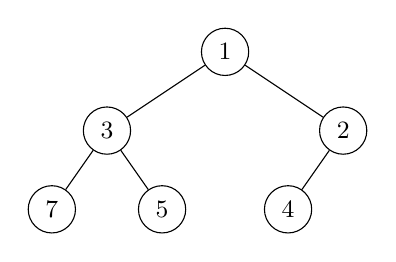
\begin{tikzpicture}[x=1cm,y=1cm,v/.style={circle,draw,minimum size=6mm,inner sep=0pt,font=\small}]
\node[v] (a) at (0,0) {1};
\node[v] (b) at (-1.5,-1) {3}; \node[v] (c) at (1.5,-1) {2};
\node[v] (d) at (-2.2,-2) {7}; \node[v] (e) at (-0.8,-2) {5}; \node[v] (f) at (0.8,-2) {4};
\draw (a)--(b) (a)--(c) (b)--(d) (b)--(e) (c)--(f);
\end{tikzpicture}
\end{center}
檢查：$1 \le 3$、$1 \le 2$；$3 \le 7$、$3 \le 5$；$2 \le 4$。 最後一層的 $7, 5, 4$ 從左邊連續填，是完全
二元樹。 注意堆積只規定父子的大小，兄弟、堂兄弟之間沒有順序：$3$ 在左、$2$ 在右也可以。

\textbf{不是最小堆積的例子}。 $\langle 1, 3, 2, 7, 5, 4 \rangle$ 把 $5$ 換成 $0$ 就不是（$3 > 0$）；
如果 $2$ 只有右孩子 $4$、沒有左孩子，也不是（不是完全二元樹）。
\end{pastsoln}
